
%\begin{figure}[t]
%\centering
%\includegraphics[scale=1,clip]{figure/n2n.eps}\vspace*{-3ex}
% \caption{Merging technique}\vspace*{-3.5ex}
% \label{fig:n2n}
%\end{figure}

\section{Discussion and Future Work}
\label{sec:discuss}

We next discuss issues in our approach and describe how we address
these issues in our future work.

\subsection{Testing Translation of Programming Languages with Fundamental Differences} Some programming languages may have much more different code structures than Java and C\# do, and existing translation tools between these programming languages may fail to translate some different code structures. Daniel \emph{et al.}~\citep{daniel2007automated} propose an approach that tests refactoring engines by comparing their refactored results given the same generated abstract syntax trees. In future work, we plan to adapt their approach to test translation tools by comparing their translation results given the same code structures as inputs. As pointed out by Waters~\citep{waters1988program}, when a source language is fundamentally different from its target language, programmers may even have to abstract a source program and to re-implement its target program from scratch. Still, API differences are important for programmers to avoid related defects when they re-implement a target program. Ravitch \emph{et al.}~\citep{RavitchJAL09} proposed an
approach that can generate bindings to expose low-level languages to high-level languages. To detect such differences, we plan to adapt their wrappers to test mapped API elements between two fundamentally different languages in future work.

\subsection{Improving Translation Tools and Detecting Related Defects} Our evaluation reveals that existing translation tools typically translate only a small number of API elements, and cannot fix many behavioral differences. Our previous work~\citep{zhong2010mining} can mine more mapping relations automatically, but mined mapping relations may also fail to fix specific behavioral differences. In future work, we plan to extend our previous work~\citep{zhong2010mining} for mining better mapping relations that can fix these differences. In addition, to investigate whether found behavioral differences introduce defects in true practice, we plan to conduct empirical studies on existing translated applications, and to propose corresponding defect-detection techniques if such defects are found in future work.

\subsection{Detecting More Behavioral Difference of Mapped API Elements} Although our approach detected many behavioral differences, it may fail to reveal all behaviors. To detect more behavioral differences, some directions seem to be promising: (1) we can rely on side effects or  mock objects to test methods without return values; (2) to test API methods that return random values, we can check the distribution of their returned values; (3) other tools such as CUTE~\citep{koushik:cute} and JPF~\citep{visser2003mcp} may help generate more test cases to reveal more behaviors; (4) our previous work~\citep{thummalapenta09:mseqgen} can generate more complicated method sequences. We plan to explore these directions in future work. In addition, our approach does not cover some types of API elements (\emph{e.g.}, abstract classes and protected elements). To test these elements, we plan to extend our wrappers in future work (\emph{e.g.}, generating a concrete wrapper class for each abstract class). In our project website, we released all synthesized and translated wrappers, so that other researchers can also employ other static/dynamic techniques to detect more behavioral differences.



%\textbf{Testing API mapping of single language.} We find that many existing approaches translate applications within single languages. For example, twinning~\citep{nita2010using} translates applications based on mapping relations of API invocations from different API libraries, and CatchUp!~\citep{henkel2005catchup} translates applications based on mapping relations of API invocations from different versions. In future work, we plan to adapt our approach to test mapping relations of API invocations within single languages. 